\chapter{ATLOD: A Terrain Level of Detail (Renderer)}
This chapter describes \textit{ATLOD} (short for \textbf{A} \textbf{T}errain \textbf{L}evel \textbf{o}f \textbf{D}etail (Renderer)), the demo terrain rendering application.
The implemented algorithm is mainly based on GeoMipMapping, but also draws some inspiration from GPU-based Geometry Clipmaps and other algorithms,
notably in its effective usage of the GPU. 

\section{Preliminaries}
\subsection{Used Technologies}
ATLOD is written in C++17 and OpenGL 4.2.
For compiling build files, CMake (minimum version 3.5) is used.
ATLOD uses the following third-party libraries:
\begin{itemize}
  \item GLM: The \textit{OpenGL Mathematics (GLM)} library provides functionality for the mathematics of graphics programming, such as classes for vectors, matrices and perspective transformations.
  \item GLEW: The \textit{OpenGL Extension Wranger Library (GLEW)} is an extension loading library for OpenGL. 
  \item GLFW: \textit{GLFW} is a multi-platform library for desktop-based OpenGL applications, offering an API for managing windows, contexts and input handling.
  \item ImGui: \textit{Dear ImGui} is a multi-platform graphical user interface library developed by Omar Cornut TODO cite.
  \item STB: STB is a collection of header-only libraries developed by Sean Barrett TODO cite. ATLOD uses \texttt{stb\_image.h} for loading images of heightmaps and textures.
\end{itemize}

ATLOD was developed with Qt Creator 9.6.1. The source code is hosted on GitHub on the repository AmarTabakovic/3d-terrain-with-lod
and is licensed under TODO.

\section{Basic Setup and Architecture}
\subsection{Overview}
TODO High-level class diagram

\subsection{Shaders}
The class \texttt{Shader} encapsulates a shader program consisting of a vertex shader and a fragment shader.
It's based on the ``Shaders'' chapter in \textit{Learn OpenGL - Graphics Programming} \cite{learnopengl}.

\subsection{Camera}
The camera class is based on the ``Camera'' chapter in \textit{Learn OpenGL - Graphics Programming} \cite{learnopengl}.
The camera is defined by its yaw and pitch angles, which are used to construct the front, up and right 
camera vectors. The camera also consists of its position, of its near and far $z$-values, of its aspect ratio,
zoom, and of its flight and look-around velocities. The aspect ratio, near and far values and zoom are used to 

\subsubsection{Automatic Flying and Rotation}
ATLOD supports automatic flying of the camera using two given world-space coordinates.
The coordinates can be entered in a dialogue window and the flight velocity is adjustable with a slider.

The flying is implemented by linearly interpolating between the starting coordinate $\mathbf{p}_{start}$ 
and the end coordinate $\mathbf{p}_{end}$ with an interpolation factor $t$ in the main game loop.
More precisely, the direction is calculated by precomputing the direction vector $\mathbf{v}_{flyDir} = \mathbf{p}_{end} - \mathbf{p}_{start}$ and then by calculating
\begin{align*}
  \mathbf{p}_{new} = \mathbf{p}_{start} + t \cdot \mathbf{v}_{flyDir}.
\end{align*}
The interpolation factor $t$ starts at 0 and gets increased by a small value $0< t_{step}\leq1$ every frame until 
$t = 1$. This $t_{step}$ is adjustable by the user and corresponds to the previously mentioned flight velocity.

The class \texttt{Camera} contains a method \texttt{lerpFly()} which gets called each frame and performs the above calculation, as shown in listing \ref{lst:lerpfly}.
\begin{lstlisting}[
  language={C++},
  label={lst:lerpfly}
  caption={Method \texttt{Camera::lerpFly()} that linearly interpolates between $\mathbf{p}_{start}$ and $\mathbf{p}_{end}$.}]
void Camera::lerpFly(float lerpFactor)
{     
    _position = origin + direction * lerpFactor;
}
\end{lstlisting}

The main render loop contains the snippet shown in listing \ref{lst:mainloopcam}
\begin{lstlisting}[
  language={C++},
  label={lst:mainloopcam}
  caption={Snippet in the main render loop that is responsible for flying.}]
float posLerp = 0.0f;
// ...
void run() {
    while (!glfwWindowShouldClose(window)) {
        // ...
        if (camera.isFlying) {
            camera.lerpFly(posLerp);
            posLerp += 0.0005 + flightVel / 50000;

            if (posLerp >= 1.0f) {
                camera.isFlying = false;
                posLerp = 0.0f;
            }
        }
        // ...
    }
}
\end{lstlisting}

The automatic camera rotation works similarly, but interpolates from the initial yaw $yaw_{init}$ to
$yaw_{init} + 2\pi$ with
\begin{align*}
  yaw_{new} = yaw_{init} + t \cdot 2\pi. 
\end{align*}

\subsection{Skybox}
A \textit{skybox} is a box in world space that simulates the sky using
six texture images, one for each side of the box. 
Skyboxes are rendered with \textit{cubemaps}

The skybox implemented in ATLOD is based on the ``Cubemaps'' section in the ``Advanced OpenGL'' chapter in \textit{Learn OpenGL - Graphics Programming} \cite{learnopengl}.
It is encapsulated in the class \texttt{Skybox}.


An improvement over the current skybox would be to actually calculate the \textit{atmospheric scattering},
which would deliver a more realistic and flexible daytime-based lighting.
A suitable approach would be \textit{precomputed atmospheric scattering} by Bruneton and Neyret \cite{precomputedatmosphericscattering}.

\subsection{Base Terrain}
The base \texttt{Terrain} class is the superclass of all terrain LOD algorithms and 
contains fields that are common between different terrain LOD algorithms,
such as the heightmap, shader, width, height, and more.
It also contains the three virtual methods \texttt{loadBuffers}, \texttt{render()}
and \texttt{unloadBuffers()}, which all terrain subclasses must implement.

The base terrain is structured as shown in listing TODO.

\subsection{Heightmaps}
The class \texttt{Heightmap} represents a heightmap and its data.
Like many game engines today, such as Unity and Unreal Engine, ATLOD supports heightmaps as 16-bit grayscale PNG images, which allow for 
strorage of up to $2^{16}-1=65535$ height values per pixel. 

\subsubsection{Heightmap Preprocessing}
Digital elevation model (DEM) data is commonly offered in the GeoTIFF file format by various DEM providers,
such as SwissTopo and OpenTopography.
GeoTIFF files can be converted into PNG using GIS software, such as 
QGIS or GDAL. 

A small Python 3 command line utility named \texttt{geotiff-to-png} for converting GeoTIFF files into 16-bit grayscale PNG images
is available in the repository of ATLOD in the \texttt{scripts} folder. 

\subsubsection{Loading}
The method \texttt{load()} is responsible for loading a heightmap
located at a given file path \texttt{fileName}.
Depending on the file extension of \texttt{fileName}, 
TODO.

The height values are stored in the field \texttt{\_data} of type \texttt{std::vector<unsigned short>}.

For terrain LOD algorithms using heightmap displacement inside the vertex shader, 
the \texttt{load()} method offers the possibility to optionally load the heightmap 
directly into an OpenGL texture object. The ID is stored on the current \texttt{Heightmap}
instance in the field \texttt{\_heightmapTextureId}, so that multiple different 
\texttt{Terrain} instances can share the same heightmap if needed.

\section{Naive Brute-force Algorithm}
The naive brute-force algorithm, which simply renders every vertex without any LOD considerations, is encapsulated in the class \texttt{NaiveRenderer}.

\subsection{Vertex and Index Organisation}
A vertex consists of its $(x,y,z)$-position,
its normal vector $(n_x,n_y,n_z)$ and of its
texture coordinates $(u,v)$. All components
are 4-byte floating point values, which means that 
per vertex, $4 \times 8 = 32$ bytes of GPU memory
get allocated. These attributes are organized 
in a vertex array object stored in the field \texttt{\_vao}.

The indices are organized such that they can be rendered as triangle strips with \texttt{GL\_TRIANGLE\_STRIPS}.
Each row is separated using a special marker index named \texttt{RESTART}, which is set to the maximum possible \texttt{GLuint} value and is used for the \texttt{GL\_PRIMITIVE\_RESTART} mode,
allowing for the entire terrain to be rendered in a single \texttt{glDrawElements()} call. This draw call happens every frame in the 
method \texttt{render()}. Figure~\ref{fig:naive-triangles} shows the organization of indices for rendering the terrain as triangle strips.

\begin{figure}[H]
  \centering
  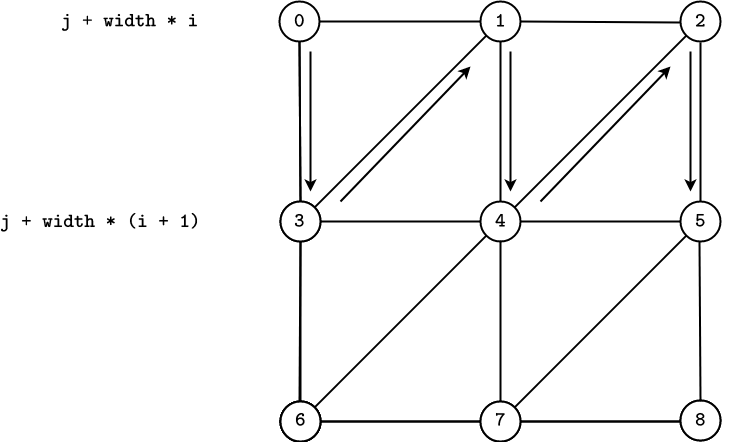
\includegraphics[width=0.9\textwidth]{atlod-naive-triangles}
  \caption{Example of a terrain layout for triangle strips. The looping index \texttt{i} goes from 0 to the terrain height and \texttt{j} from 0 to the terrain width. The final indices to be rendered are 0,3,1,4,2,5,\texttt{RESTART},3,6,4,7,5,8,\texttt{RESTART}.}\label{fig:naive-triangles}
\end{figure}

\subsubsection{Loading}
The method \texttt{loadBuffers()} is responsible for loading the data into the vertex and index buffer.
The first step is the generation of the normal vectors. This is done in the method \texttt{loadNormals},
where the normals of each vertex are calculated into an intermediate vector \texttt{\_normals}.

The normals are calculated as follows. Each vertex consists 
of its $\mathbf{p}_{pos} = (x,y,z)$ position, where the $(x,z)$-coordinates
are given by the current position relative to the heightmap size and the $y$-coordinate is retrieved from the heightmap in memory.
The four orhogonally neighboring points 

Geometrically, the direction of a sum of vectors is given by 
constructing a chain of these vectors, such that the 
beginning of the next vector is at the tip of the previous vector,
and then ``walking'' along all vectors from the first to the last vector.

\subsection{Shading}
The shading is calculated with the Phong shading technique in the fragment shader.

\section{GeoMipMapping}
The implementation supports most basic functionalities described in the original paper, but differs in a few key aspects.
It also draws some inspiration from other approaches, most notably from GPU-based Geometry Clipmaps by Hoppe and Asirvatham
and from ``Terrain Rendering in Frostbite Using Procedural Shader Splatting'' by Andersson for the Frostbite game engine TODO cite.
Both approaches utilize a single flat mesh (positioned around the viewer in Hoppe and Asirvatham's approach) and store the heightmap as a texture object. The height values are sampled in the vertex shader, which are then 
used to displace the flat mesh on the $y$-axis. 

The idea of using a texture object for the heightmap is applied to ATLOD's GeoMipMapping implementation.
Rather than generating vertex buffers for each block and loading in the height values into the vertices directly (as in the naive renderer implementation),
a single flat mesh with the side length of the block size is generated once at load time. At render time, for each block the mesh is translated 
to the block's world-space position and the height values get sampled from the heightmap, which is stored as a texture object.
The upcoming subsections describe the approach in greater detail.

\subsection{Block Structure}
As described in the high-level overview of the GeoMipMapping algorithm, 
the algorithm splits up the terrain into square blocks of side length $2^n+1$.

In this implementation, a block is the structure containing information of a
particular section of the terrain. The class \texttt{GeoMipMappingBlock}
represents such a block and contains the following fields:
\begin{itemize}
  \item \texttt{unsigned \_blockId}: this field stores the ID of the current block.
  \item \texttt{unsigned \_currentBorderBitmap}: this field stores the current border permutation as a bitmap.
  \item \texttt{float \_minY} and \texttt{float \_maxY}: these two fields store the minimum and maximum $y$-coordinates of that particular block.
  \item \texttt{glm::vec2 \_translation}: this field stores the 2-dimensional translation vector for translating the flat mesh to the block's actual position.
  \item \texttt{glm::vec3 \_aabbCenter} and \texttt{glm::vec3 \_trueCenter}: \texttt{\_aabbCenter} stores the position of the center of the AABB of the block, i.e. its $y$-coordinate is set to $\texttt{\_maxY} - \texttt{\_minY}$.
        This field is used for view-frustum culling during rendering.
        The field \texttt{\_trueCenter} on the other hand stores the actual center position of that block in world-space, i.e. its $y$-coordinate is computed from the heightmap. 
        This field is used for the distance calculation for the LOD determination during rendering.
\end{itemize}

\subsection{Vertex and Index Organisation}
ATLOD's GeoMipMapping implementation consists of a single vertex buffer and index buffer.
The vertex buffer contains the vertices for a single flat $b \times b$ mesh centered around $(0,0,0)$, where $b = 2^n + 1$ is the block size and $n$ is the maximum LOD level.
The vertices of the flat mesh only consist of 4-byte floating point $(x,z)$-coordinates, since the mesh is flat.

The index buffer contains the 4-byte unsigned integer indices of the flat mesh and is organized as follows:
the flat mesh is split up into its border area and center area.
The reason for splitting the mesh up this way will be made clear shortly.
The first part of the index buffer stores the indices of the border area
for every LOD level and border permutation, and
the second part of the index buffer stores the center area for every LOD level. 
What a \textit{border permutation} is will be explain in the next section.
Figure \ref{fig:atlod-geomipmapping-index-buffers} shows the described index buffer 
organisation.

\begin{figure}[H]
  \centering
  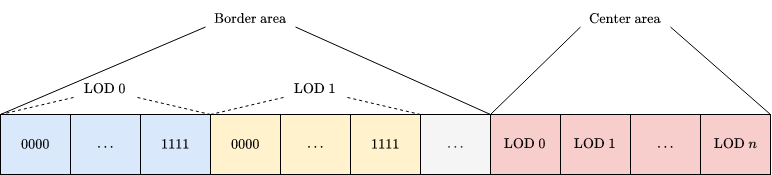
\includegraphics[width=1.0\textwidth]{atlod-geomipmapping-index-buffer.png}
  \caption{The index buffer organisation of the single flat block. The variable $n$ corresponds to the maximum LOD level.}\label{fig:atlod-geomipmapping-index-buffers}
\end{figure}

\subsubsection{Border Permutations}
A border permutation is defined to be a 4-tuple $(t,b,l,r)$,
where $t,b,l,r$ correspond to top, bottom, left and right, and where each entry is set to 1 if the block on 
the corresponding side has a lower LOD, and 0 otherwise. For example, if the top and right neighboring blocks
have a lower LOD than the current block, the border permutation is $(1,0,0,1)$.
These border permutations can also be expressed as bitfields, e.g. \texttt{1001},
which allows for easy indexing into the subset of the index buffer containing the relevant indices.
The number of possible permutations is $2^4=16$.
In order for this approach to work, the difference in LOD level between any two bordering blocks 
must be at most 1. 
A similar approach is described by Andersson in SIGGRAPH 2007 for the terrain rendering 
in the Frostbite game engine for the game Battlefield 2, with their approach requiring only 9 permutations.
Figure \ref{fig:atlod-geomipmapping-crack-avoidance} shows all possible border permutations of a $5 \times 5$ block at LOD level 2.

\begin{figure}[H]
  \centering
  \subfloat[\centering \texttt{0000}.]{{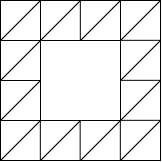
\includegraphics[width=0.17\textwidth]{atlod-geomipmapping-0000.png} }}
  \qquad
  \subfloat[\centering \texttt{0001}.]{{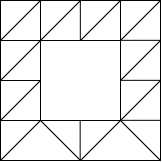
\includegraphics[width=0.17\textwidth]{atlod-geomipmapping-0001.png} }}
  \qquad
  \subfloat[\centering \texttt{0010}.]{{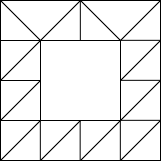
\includegraphics[width=0.17\textwidth]{atlod-geomipmapping-0010.png} }}
  \qquad
  \subfloat[\centering \texttt{0011}.]{{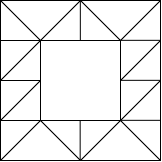
\includegraphics[width=0.17\textwidth]{atlod-geomipmapping-0011.png} }}

  \subfloat[\centering \texttt{0100}.]{{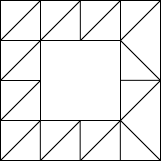
\includegraphics[width=0.17\textwidth]{atlod-geomipmapping-0100.png} }}
  \qquad
  \subfloat[\centering \texttt{0101}.]{{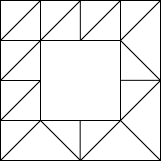
\includegraphics[width=0.17\textwidth]{atlod-geomipmapping-0101.png} }}
  \qquad
  \subfloat[\centering \texttt{0110}.]{{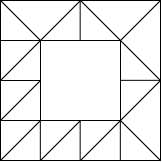
\includegraphics[width=0.17\textwidth]{atlod-geomipmapping-0110.png} }}
  \qquad
  \subfloat[\centering \texttt{0111}.]{{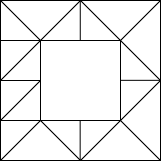
\includegraphics[width=0.17\textwidth]{atlod-geomipmapping-0111.png} }}

  \subfloat[\centering \texttt{1000}.]{{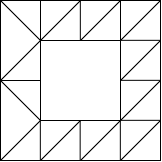
\includegraphics[width=0.17\textwidth]{atlod-geomipmapping-1000.png} }}
  \qquad
  \subfloat[\centering \texttt{1001}.]{{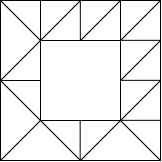
\includegraphics[width=0.17\textwidth]{atlod-geomipmapping-1001.png} }}
  \qquad
  \subfloat[\centering \texttt{1010}.]{{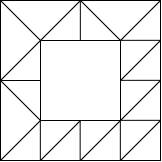
\includegraphics[width=0.17\textwidth]{atlod-geomipmapping-1010.png} }}
  \qquad
  \subfloat[\centering \texttt{1011}.]{{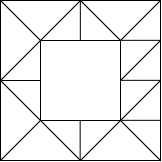
\includegraphics[width=0.17\textwidth]{atlod-geomipmapping-1011.png} }}

  \subfloat[\centering \texttt{1100}.]{{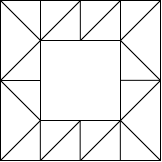
\includegraphics[width=0.17\textwidth]{atlod-geomipmapping-1100.png} }}
  \qquad
  \subfloat[\centering \texttt{1101}.]{{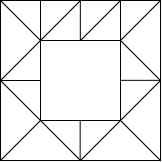
\includegraphics[width=0.17\textwidth]{atlod-geomipmapping-1101.png} }}
  \qquad
  \subfloat[\centering \texttt{1110}.]{{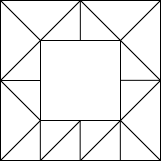
\includegraphics[width=0.17\textwidth]{atlod-geomipmapping-1110.png} }}
  \qquad
  \subfloat[\centering \texttt{1111}.]{{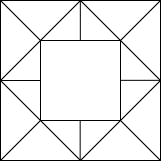
\includegraphics[width=0.17\textwidth]{atlod-geomipmapping-1111.png} }}
  \caption{Every possible border permutation for a LOD 2 GeoMipMap of a $5 \times 5$ block. The center subblocks have been omitted from the illustration.}\label{fig:atlod-geomipmapping-crack-avoidance}
\end{figure}

This makes clear why the flat mesh is split into its border and center area.
The center area only depends on the LOD level and is the same 
regardless of the current border permutation. 
Not splitting the flat mesh up into its border and center area 
would require longer index buffer generation times and consume 
significantly more GPU memory.

\subsubsection{Starts and Sizes Lists}
The organisation of the index buffer as presented requires some additional
management of the start indices and sizes of the subsets of the index buffer. The \texttt{GeoMipMapping} class 
contains four members of the type \texttt{std::vector<unsigned>}:
\texttt{\_borderStarts}, \texttt{\_borderSizes}, \texttt{\_centerStarts} and \texttt{\_centerSizes}.
The \texttt{\_borderStarts} and \texttt{\_borderSizes} lists store the starting index 
(into the index buffer) and 
the number of indices, for a subset of the index buffer containing the indices of the border area for a given border permutation and LOD level.
Both the lists are indexed by multiplying the current LOD level by 16 
and then adding the current border permutation to it.
The \texttt{\_centerStarts} and \texttt{\_centerSizes} lists are indexed similarly,
except that they are indexed simply with the current LOD level.

In order to illustrate the idea more clearly, the following example is given:
say that the current block has a LOD level of 1 and every neighboring block has the 
same LOD level (i.e. the border permutation is $(0,0,0,0)$). 
We want to render the block, which means 
we need to retrieve the indices for the flat mesh 
at the LOD level 1 and for the border permutation \texttt{0000}.
The start index and the size for the border area are retrieved with \texttt{\_borderStarts[1 * 16 + 0b0000]}
and \texttt{\_borderSizes[1 * 16 + 0b0000]} respectively, and for 
the center area with \texttt{\_centerStarts[1]} and \texttt{\_centerSizes[1]}.
These four values are passed to the two \texttt{glDrawElements()} draw calls for the block,
which renders the flat mesh at the chosen LOD level 1 and border permutation $(0,0,0,0)$.
The full rendering process is described in the subsection ``Rendering'' of this section.
Figure \ref{fig:atlod-starts-sizes-example} illustrates this example.

\begin{figure}[H]
  \centering
  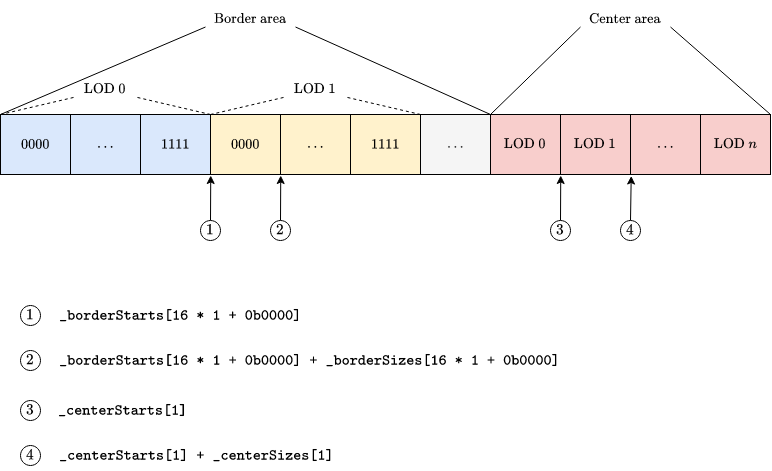
\includegraphics[width=1.0\textwidth]{atlod-starts-sizes-example.png}
  \caption{Illustration of accessing the start index and size of the subsets of the index buffer for LOD 1 and border permutation $(0,0,0,0)$}\label{fig:atlod-starts-sizes-example}
\end{figure}

\subsubsection{Loading}
Now that the organisation of the vertices and indices 
has been presented, the loading mechanisms are described.
The vertex and index buffers get loaded in the method \texttt{loadBuffers()},
which calls the two helper methods \texttt{loadVertices()} an \texttt{loadIndices()}.

The method \texttt{loadVertices()} simply generates the vertex array object with its ID stored in the field \texttt{\_vao}
and loads the vertices of the flat mesh of size $blockSize \times blockSize$
centered around $(0,0,0)$ into a vertex buffer with its ID stored in the field \texttt{\_vbo}.
\begin{lstlisting}[
  language=C++,
  caption={Method \texttt{GeoMipMapping::loadVertices()} that generates the vertex array object and loads the
  vertex buffer with the flat mesh of size $blockSize \times blockSize$ centered around $(0,0,0)$.}]
void GeoMipMapping::loadVertices()
{
    for (int i = 0; i < _blockSize; i++) {
        for (int j = 0; j < _blockSize; j++) {
            // Load vertices around center point 
            float x = (-(float)_blockSize / 2.0f + (float)_blockSize * j / (float)_blockSize);
            float z = (-(float)_blockSize / 2.0f + (float)_blockSize * i / (float)_blockSize);

            _vertices.push_back(x); // Position x 
            _vertices.push_back(z); / Position z 
        }
    }

    glGenVertexArrays(1, &_vao);
    glBindVertexArray(_vao);

    glGenBuffers(1, &_vbo);
    glBindBuffer(GL_ARRAY_BUFFER, _vbo);
    glBufferData(GL_ARRAY_BUFFER, _vertices.size() * sizeof(float), &_vertices[0], GL_STATIC_DRAW);

    // Position attribute
    glVertexAttribPointer(0, 2, GL_FLOAT, GL_FALSE, 2 * sizeof(float), (void*)0);
    glEnableVertexAttribArray(0);
}
\end{lstlisting}

The index loading mechanism is more complex.
The top-level index loading method \texttt{loadIndices()}
performs the following operations:
\begin{itemize}
  \item It loads the LOD 0 and LOD 1 representation of the flat mesh using \texttt{loadLod0()} and \texttt{loadLod1()} respectively. The LOD 0 and LOD 1 indices require special treatment. They are stored as borders and do not have a center.
  \item It loads the rest of the indices from LOD 2 to the maximum LOD level, by first loading in the border indices with \texttt{loadBorderAreaForLod()}
        and then the center areas with \texttt{loadCenterAreaForLod()}.
\end{itemize}

\subsection{LOD Selection}
The LOD of ATLOD's GeoMipMapping implementation is based on the Euclidean distance $dist$ between 
the camera's position $\mathbf{p}_{camPos} = (camPos_x, camPos_y, camPos_z)$ 
and the block's center point $\mathbf{p}_{blockCenter} = (blockCenter_x, blockCenter_y, blockCenter_z)$
\begin{align*}
  dist = \sqrt{ \begin{aligned} & (blockCenter_x - camPos_x)^2 + (blockCenter_y - camPos_y)^2 \\
          & + (blockCenter_z-camPos_z)^2 \end{aligned}}.
\end{align*}
A minor optimization for this calculation is possible by instead calculating the LOD using the squared distance, 
which avoids an expensive square-root call.

Two different LOD determination modes are possible: the \textit{linearly growing distance} and the \textit{exponentially growing distance}.
Both use a base distance value $baseDist$ which 
can be set by the user. Note that $baseDist$ should be larger than $blockSize$,
as otherwise cracks in the terrain may occur, but also not too large, 
so that the performance is still adequate.
The LOD computed by the linearly growing distance can be defined with the following recursive formula
\begin{align*}
  lod_{lin}(dist, i) = 
  \begin{cases}
    l - i  + 1& dist \leq i \cdot baseDist\\
    lod_{lin}(dist, i + 1) & i \cdot baseDist < dist < (l + 1) \cdot baseDist\\
    0 & \text{otherwise}
  \end{cases},
\end{align*}
where $i$ starts at 1 and $l$ is the maximum LOD level.
As a basic example, say that $l=3,baseDist=100,dist=250$.
We begin computing the LOD level with $lod_{lin}(250,1)$.
The second condition $1 \cdot 100 < 250 < 4 \cdot 100$ holds, so we continue with $lod_{lin}(250,2)$.
Again, the second condition $2 \cdot 100 < 250 < 4 \cdot 100$ holds, so we continue with $lod_{lin}(250,3)$.
Now, the first condition $250 \leq 3 \cdot 100$ holds, so the entire expression evaluates to $3-3+1=1$,
which means we set the LOD level of the block to 1.

The exponentially growing distance is defined very similarly:
\begin{align*}
  lod_{exp}(dist, i) = 
  \begin{cases}
    l - i + 1 & dist \leq i \cdot baseDist\\
    lod_{exp}(dist, 2i) & i \cdot baseDist < dist < (l+1) \cdot baseDist\\
    0 & \text{otherwise}
  \end{cases}.
\end{align*}

The above expressions are implemented in the \texttt{GeoMipMapping} class in a single method \texttt{determineLodDistance()}.
The LOD determination mode can be set with the boolean argument \texttt{doubleEachLevel}.
Additionally, the minimum and maximum LOD levels can be manually set to be different from 0 and $l$ respectively 
by the user, with the fields \texttt{\_minLod} and \texttt{\_maxLod}. 
Note that the user defined \texttt{\_minLod} and \texttt{\_maxLod} values
are both set to $\max\{0,\texttt{\_minLod}\}$ and $\min\{l,\texttt{\_maxLod}\}$ respectively in the constructor, 
so that the LOD level does not go out of bounds.
Listing \ref{lst:determineloddistance} shows the method \texttt{determineLodDistance}.

\begin{lstlisting}[
  language={C++},
  label={lst:determineloddistance},
  caption={Method \texttt{GeoMipMapping::determineLodDistance()} that determines the LOD level of a block 
  based on its distance to the camera.}]
unsigned GeoMipMapping::determineLodDistance(float squareDistance, float baseDist, bool doubleEachLevel)
{
    unsigned distancePower = 1;
    for (unsigned i = 0; i < _maxLod - _minLod; i++) {
        if (squaredDistance < distancePower * distancePower * baseDist * baseDist)
            return _maxLod - i;

        if (doubleEachLevel)
            distancePower <<= 1;
        else
            distancePower++;
    }
    return _minLod;
}
\end{lstlisting}

Figure \ref{fig:atlod-lin-exp} shows both LOD determination modes in action.
\begin{figure}[H]
  \centering
  \subfloat[\centering Linearly growing distance mode.]{{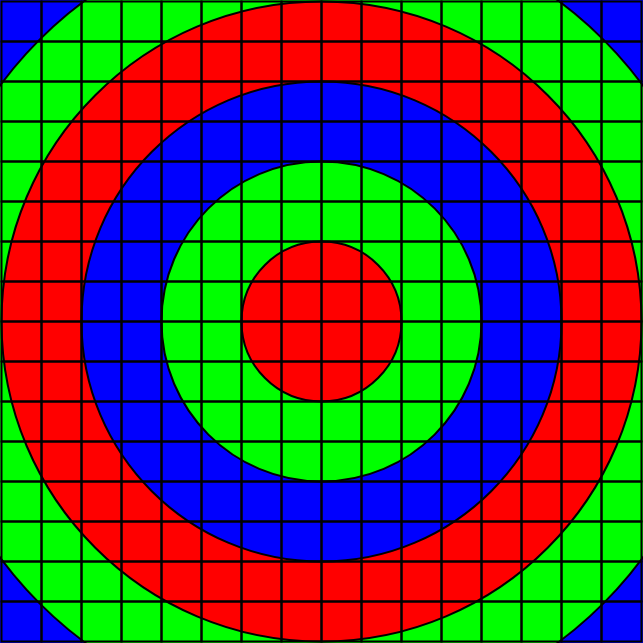
\includegraphics[width=0.4\textwidth]{atlod-lod-linear} }}
  \qquad
  \subfloat[\centering Exponentially growing distance mode.]{{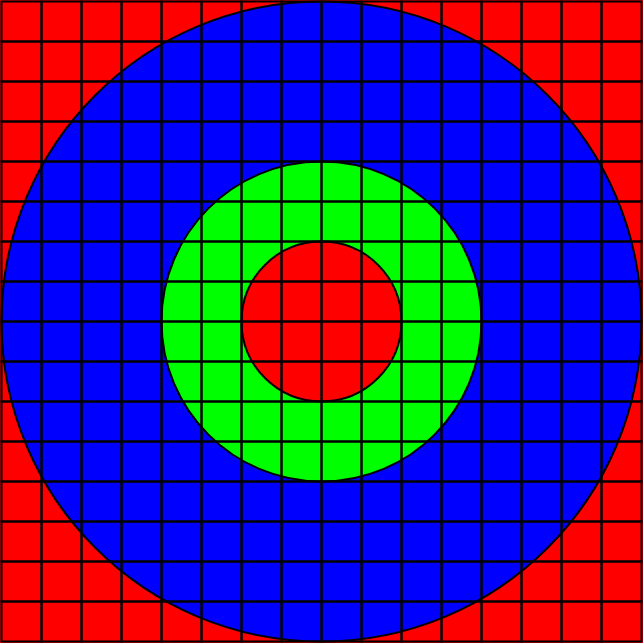
\includegraphics[width=0.4\textwidth]{atlod-lod-exponential} }}%
  \caption{Illustration of a flat terrain showcasing the linearly growing distance mode (a) and exponentially growing distance mode (b). The red, green and blue colors indicate successively lower LOD levels, starting from the maximum level in the center.}\label{fig:atlod-lin-exp}
\end{figure}

\subsection{View-frustum Culling}
View-frustum culling is implemented with the methods TODO in the \texttt{Camera} class.


\subsection{Rendering}
The method \texttt{render()} that is called each frame performs in two phases:
\begin{itemize}
  \item The first phase iterates through every block, calculates the distance between 
        the block's \texttt{\_trueCenter} and the camera's position, and updates the LOD level of the block 
        accordingly. 
  \item The second phase consists of performing view-frustum culling, setting the uniform variables in the shader,
        and finally rendering the block.
\end{itemize}

\subsubsection{Vertex Shader}
The vertex shader first translates the vertex from its initial position around $(0,0,0)$ to its actual world-space 
position using the uniform \texttt{vec2} variable \texttt{translation}.

\subsubsection{Fragment Shader}
The fragment shader 

The Phong shading is based on TODO cite and is performed with the following steps: 
first, the heightmap is sampled at the four orthogonally neighboring points $\mathbf{p}_{1,0} = (x + 1,z)$, $\mathbf{p}_{-1,0} = (x - 1,z)$, $\mathbf{p}_{0,1} = (x, z + 1)$ and $\mathbf{p}_{0,-1} = (x, z - 1)$,
where $(x,z)$ is the current texture coordinate for sampling the current height from the heightmap.
Using these four points, the slope in $x$ and $z$-direction can be calculated by computing
\begin{align*}
  dx = \mathbf{p}_{-1,0} - \mathbf{p}_{1,0}\\
  dz = \mathbf{p}_{0,-1} - \mathbf{p}_{0,1}.
\end{align*}
These values can now be used to create a normal vector
\begin{align*}
  \mathbf{n} = \frac{(dx, 2, dz)}{\lVert(dx,2,dz)\rVert}.
\end{align*}

Listing TODO shows the calculation of the normal vector from the heightmap texture.


\subsection{Conclusion}
The implementation still has some room for improvements, such as instanced rendering, geomorphing 
and a quadtree-based frustum culling. The memory consumption by the index buffer could be 
further brought down by only defining indices for the border permutations $(0,0,0,0),
(1,1,1,1),(1,1,0,0),(1,0,1,0),$$(1,1,1,0)$ and 
by rotating the mesh about the $y$-axis such that the borders align without cracks.
